\chapter{有限元素法}

\begin{figure}[hbt!]
\begin{center}
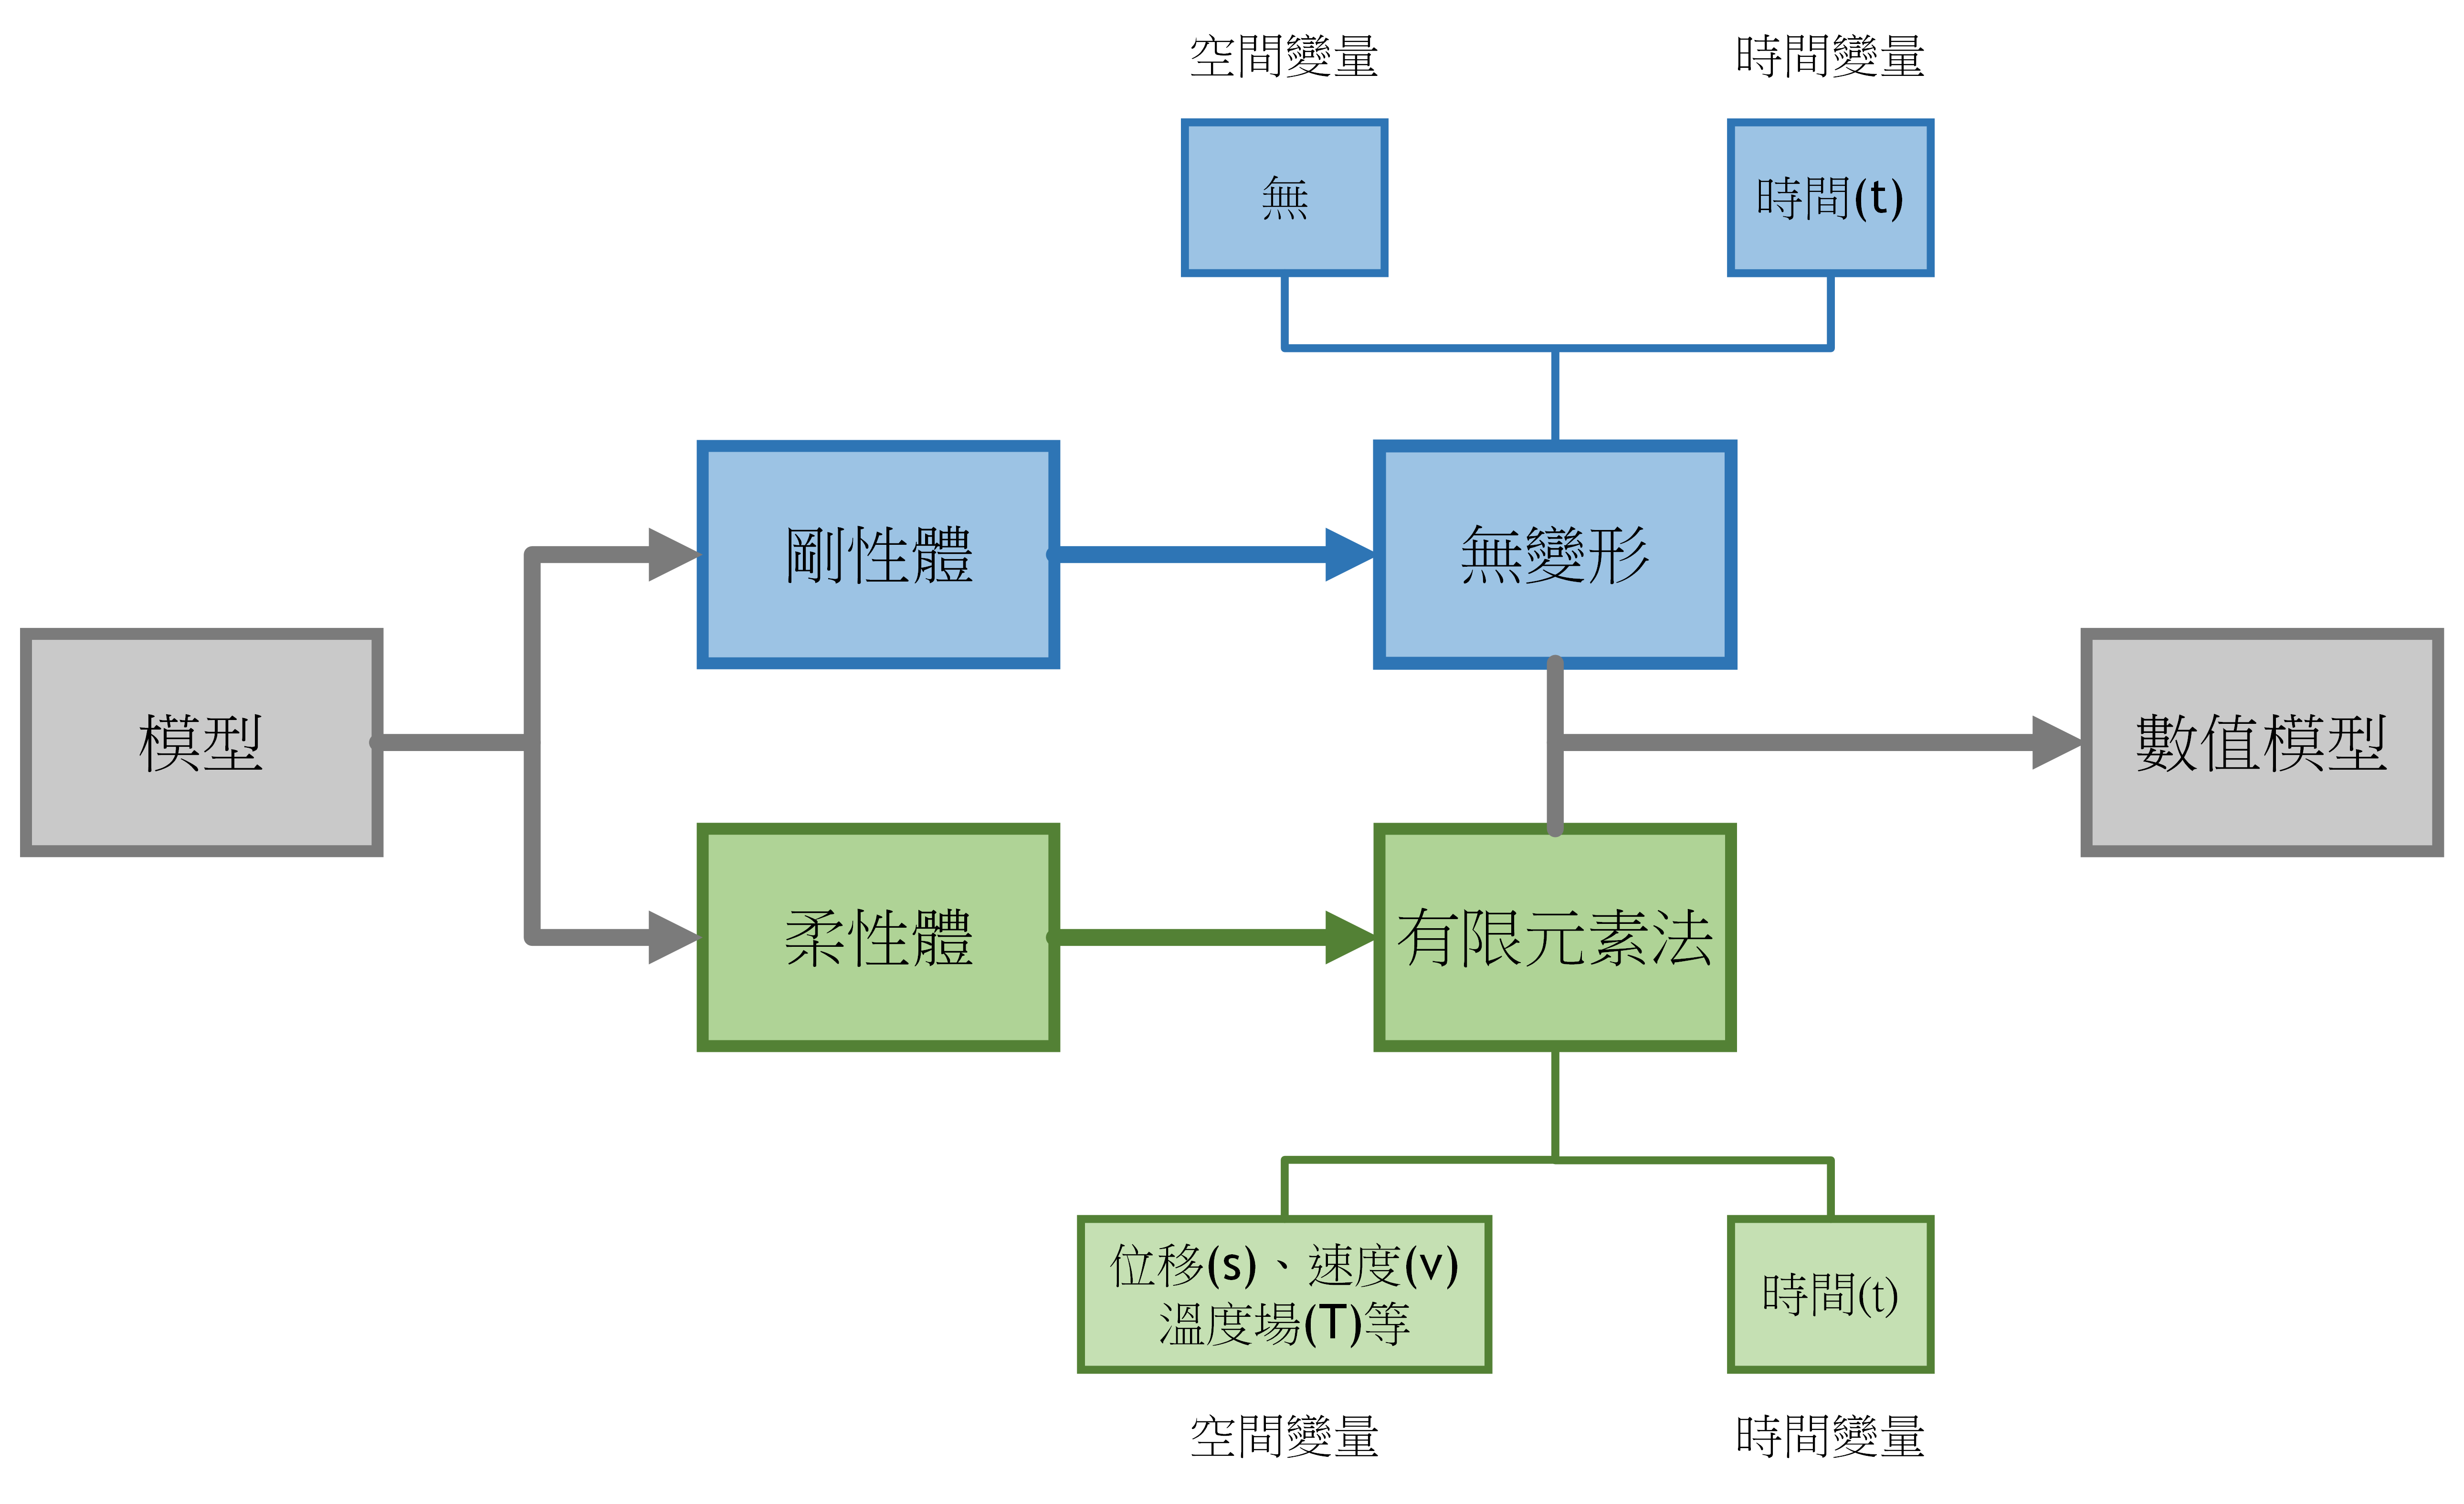
\includegraphics[width=16cm]{有限元素法}
\caption{\Large 有限元素法介紹}\label{有限元素法}
\end{center}
\end{figure}
時間及空間問題常用偏微分方程(PDE)做數值求解,將根據不同的模型進行弱化、離散化等求解,此動作稱為有限元素法(FEM),通過在模型上簡化連續變量的複雜性來實現近似求解,用於複雜的工程結構或物理系統的行為。\\
通常用在具有多種變量的模型上,在分析之前通常加設物理為剛體,剛體狀態下的模擬較為可控並且只擁有時間變量,所以使用常微分方程(ODE)及可計算。\\
而柔性體則會因為受力情況的不同而產生多種變量,才需要利用偏微分方程求解,對物體進行弱化、離散化並劃分網格如(圖 \ref{有限元素法}),接著代入方程計算,此動作稱為有限元素法。\\
\newpage
%---------------------第二章/基本概念及假設假定-------------------------%
\section{基本概念}

\begin{figure}[hbt!]
\begin{center}
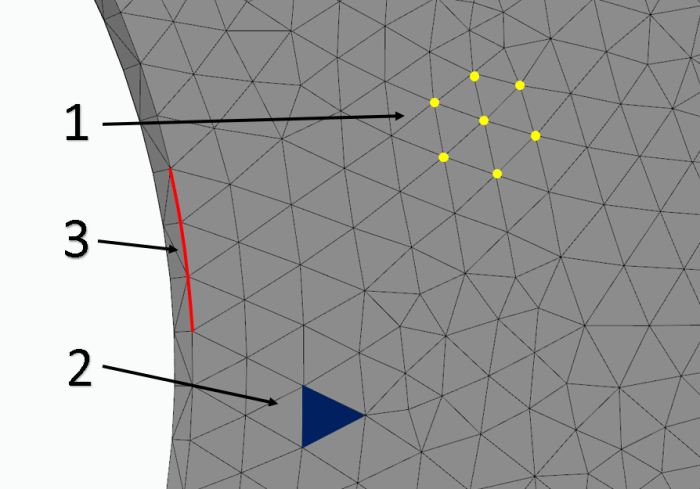
\includegraphics[width=12cm]{有限元素法介紹}
\caption{\Large 基本概念}\label{有限元素法介紹}
\end{center}
\end{figure}

\begin{enumerate}
\item 節點:每個元素的角落或中心點,用於連接元素之間的邊界條件和解決方程,如(圖 \ref{有限元素法介紹})上所箭頭1指示。
\item 元素:通常由三角形或者四邊形等形成的區域結構,如(圖 \ref{有限元素法介紹})上箭頭2所指示。
\item 邊界條件:存在於物理系統邊界如(圖 \ref{有限元素法介紹})上的約束及負荷力,模擬實際情況下的條件約束和外界影響,。
\item 自由度: 節點上變量的個數,例如位移的節點自由度為3,表示單個節點擁有三個坐標方向的位移,又例如熱分析時節點自由度為1,表示某個節點處的溫度。
\item 網格:由數個元素經由節點連接所組成,用以表示在需求解的區域上。
\item 變形:系統在外力的影響下發生的形變,經過分析後計算每個元素的變形及變形之間的相互引響預測整得系統的變形及應力、各種參數的分布。
\item 離散化:將物理系統或結構等連續變量通過計算轉換為數格元素的過程,目的在於減化數據,減少連續變量的複雜性,便於處理及分析。關於公式及步驟會因為模型或問題的類型不同而有不一樣的計算方式。
\item 材料特性:物理系統(模型)的材料性質,不同的材料其中的參數各為不同(彈性模數、蒲松比、極限強度、降伏強度等)。\\
\end{enumerate}

\subsection{邊界條件}
分為兩種邊界條件,為位移值或施加力條件。

\begin{enumerate}
\item 位移邊界條件:規定了結構或邊界上的位移及變形的特定值或關係。

\begin{itemize}
\item 固定邊界條件:也稱為約束邊界條件,令特定的某些節點或自由度的位移為零,使其無法發生位移。
\item 位移約束:指定特定節點或自由度的位移值, 可以是定值或隨時間變化的函數。
\item 斜率約束:規定特定節點的自由度的位移斜率(導數),用於描述特定邊界上的傾斜或旋轉。
\end{itemize}

\item 力邊界條件:規定了結構或邊界上施加的外部力或力的分布。

\begin{itemize}
\item 負荷:施加在結構上的集中力或分布力,可以是靜態或動態負荷。
\item 壓力:施加在邊界上的或表面力,可以是均勻或非均勻的。
\item 動力學條件:施加在結構上的動態加載。\
\end{itemize}
\end{enumerate}
\newpage

\subsection{網格劃分基本原則}
\begin{enumerate}
\item 網格數量:將決定計算精度及規模大小,一般狀況中,網格數量增加計算精度也會跟著提升,但伴隨而來的是更大的計算量,所以在制定網格大小時應權衡兩個因素。
\item 網格疏密:在某些變化梯度較大的部位(應力集中處),需要大密集的網格,密集往個將更好反映數據變化,反之變化梯度較小的部位則用較稀疏的網格,而不同單元之間的連接則採用特殊的過度單元或多點約束等方法連接,才能更好的分配資源,兼顧計算量何計算精度。
\item 網格質量:指網格形狀的合理性,質量的好壞將直接影響計算精度,質量較差的除了造成局部的計算精度偏差甚至會直接終止計算,因此在重要部位時應該確保其擁有高品質的表現。
如果網格都是由等邊三角形、正方形、正四面體、立方六面體等組成,則求解精度可以非常接近實際值,但這種只存在於理想狀態下,實際運用卻很難做到。\
\end{enumerate}

\begin{itemize}
\item 元素質量評價指標
\end{itemize}

\begin{enumerate}
\item 單元的邊長比、面積比及體積比,理想的邊長比為1,以正三角形、正四面體、正六面體為參考基準。
\item 扭曲度:單元內部扭轉及面外的翹曲程度。
\item 疏密過渡:應力梯度方向和橫向過渡情況,應力集中部分應較為密集,則反之。
\item 節點、元素排部:合理的節點及元素有助於帶入方程式計算,可以提高求解效率,並且須注意消除重複的節點及元素。
\end{enumerate}
下列(圖 \ref{網格1mm-1})至(圖 \ref{網格50mm-2})為網格疏密不同造成的分析差\

\begin{figure}[htbp]
  \centering
  \begin{minipage}{0.45\textwidth}
    \centering
    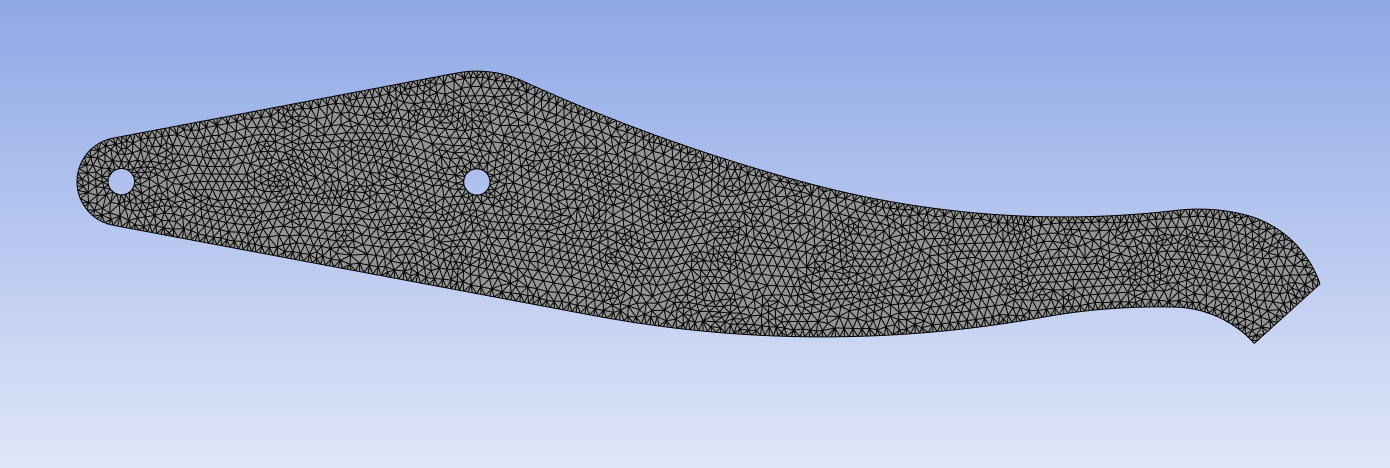
\includegraphics[width=\textwidth]{網格1mm-1}
    \caption{較密網格}
    \label{網格1mm-1}
  \end{minipage}
  \hfill
  \begin{minipage}{0.45\textwidth}
    \centering
    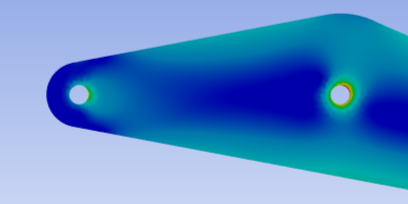
\includegraphics[width=\textwidth]{網格1mm-2}
    \caption{較密網格所得應力雲圖}
    \label{網格1mm-2}
  \end{minipage}
  
  \vspace{0.75cm} % 調整垂直間距
  
  \begin{minipage}{0.45\textwidth}
    \centering
    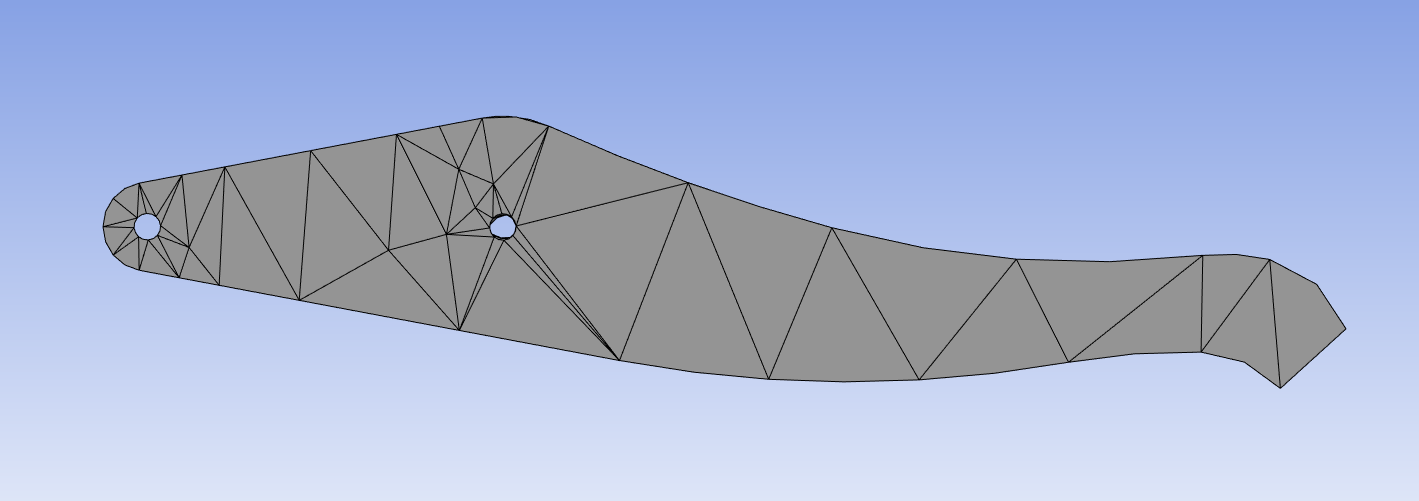
\includegraphics[width=\textwidth]{網格50mm-1}
    \caption{較粗網格}
    \label{網格50mm-1}
  \end{minipage}
  \hfill
  \begin{minipage}{0.45\textwidth}
    \centering
    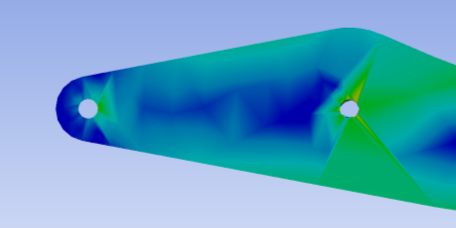
\includegraphics[width=\textwidth]{網格50mm-2}
    \caption{較粗網格所得應力雲圖}
    \label{網格50mm-2}
  \end{minipage}
\end{figure}
\newpage

%--------------------------第二章/有限元計算公式--------------------------%
\section{計算及公式介紹}
此章節主要介紹常見的結構力學的有限元計算公式及方法順序,了解到平時由電腦計算的有限元素法及代數方程式,

\subsection{變形分析}

在有限元素分析中,通常使用格拉朗日公式,透過觀察材料的平移或旋轉來建立力學方程。
在材料上設置隨意點(X),,觀察點(X)隨時間(t)變化後的材料位移矢量u(X,t),轉換為空間坐標系x=X+u即可以得到一個拉格朗日公式,只要材料為柔性體就會產生局部變化,此現象稱為應變或伸長,下列將透過多種方式來描述材料變形過程。\

\begin{itemize}
\item 變形梯度
\end{itemize}

變形梯度F定義為
$$
\mathbf{F}=\frac{\partial \mathbf{x}}{\partial \mathbf{X}}=\mathbf{I}+\frac{\partial \mathbf{u}}{\partial \mathbf{X}}
$$
其中, $\mathbf{I}$ 等同張量, 展開為矩陣形式為:\
$$
\mathbf{F}=\left[\begin{array}{lll}
\frac{\partial x}{\partial X} & \frac{\partial x}{\partial Y} & \frac{\partial x}{\partial Z} \\
\frac{\partial y}{\partial X} & \frac{\partial y}{\partial Y} & \frac{\partial y}{\partial Z} \\
\frac{\partial z}{\partial X} & \frac{\partial z}{\partial Y} & \frac{\partial z}{\partial Z}
\end{array}\right]=\left[\begin{array}{ccc}
1+\frac{\partial u}{\partial X} & \frac{\partial u}{\partial Y} & \frac{\partial u}{\partial Z} \\
\frac{\partial v}{\partial X} & 1+\frac{\partial v}{\partial Y} & \frac{\partial v}{\partial Z} \\
\frac{\partial w}{\partial X} & \frac{\partial w}{\partial Y} & 1+\frac{\partial w}{\partial Z}
\end{array}\right]
$$
上述矩陣包含材料局部旋轉和變形的完整解釋,其中還顯示許多訊息,例如:\
由於dx=FdX,未變形體dX中小線段是如何旋轉並拉伸,成為變形體dX中的線段,我們將F張量看做一個矩陣,第一列提供線段最開始沿X方向的大小和方向等信息。從數學角度來看,F是從X改變到x雅可比矩陣,因此它的行列為式J=det(F)為局體體積比例因子。對於不可壓縮材料,J=1。
極分析定理表明,任何二階張量都可以分解為純轉動和對稱張量的成績,利用這一定理將剛體轉動與變形分開:\
F=RU\
這可以解釋為先發生變形(伸長張量U),再進行剛性旋轉(旋轉矩陣R)。如此一來,如果沒有旋轉,右伸長張量則為變形梯度,因此U的解釋與F類似。\
同樣也可以將變形梯度分解為\
F=VR\
此過程中,會先發生剛體轉動,然後轉動的體發生形變,變形透過左伸長量(V)描述。
這兩個伸長張量(U)、(V)通過純轉向有著關聯,例如$\mathbf{V}=\mathbf{F R}^T=\mathbf{R} \mathbf{U} \mathbf{R}^T$。事實上,此處旋轉矩陣的轉置也是其自身的逆 $\left(\mathbf{R}^T \mathbf{R}=\mathbf{R R}^T=\mathbf{I}\right)$ 。


\subsection{應力分析}


\section{分析步驟}
\begin{figure}[hbt!]
\begin{center}
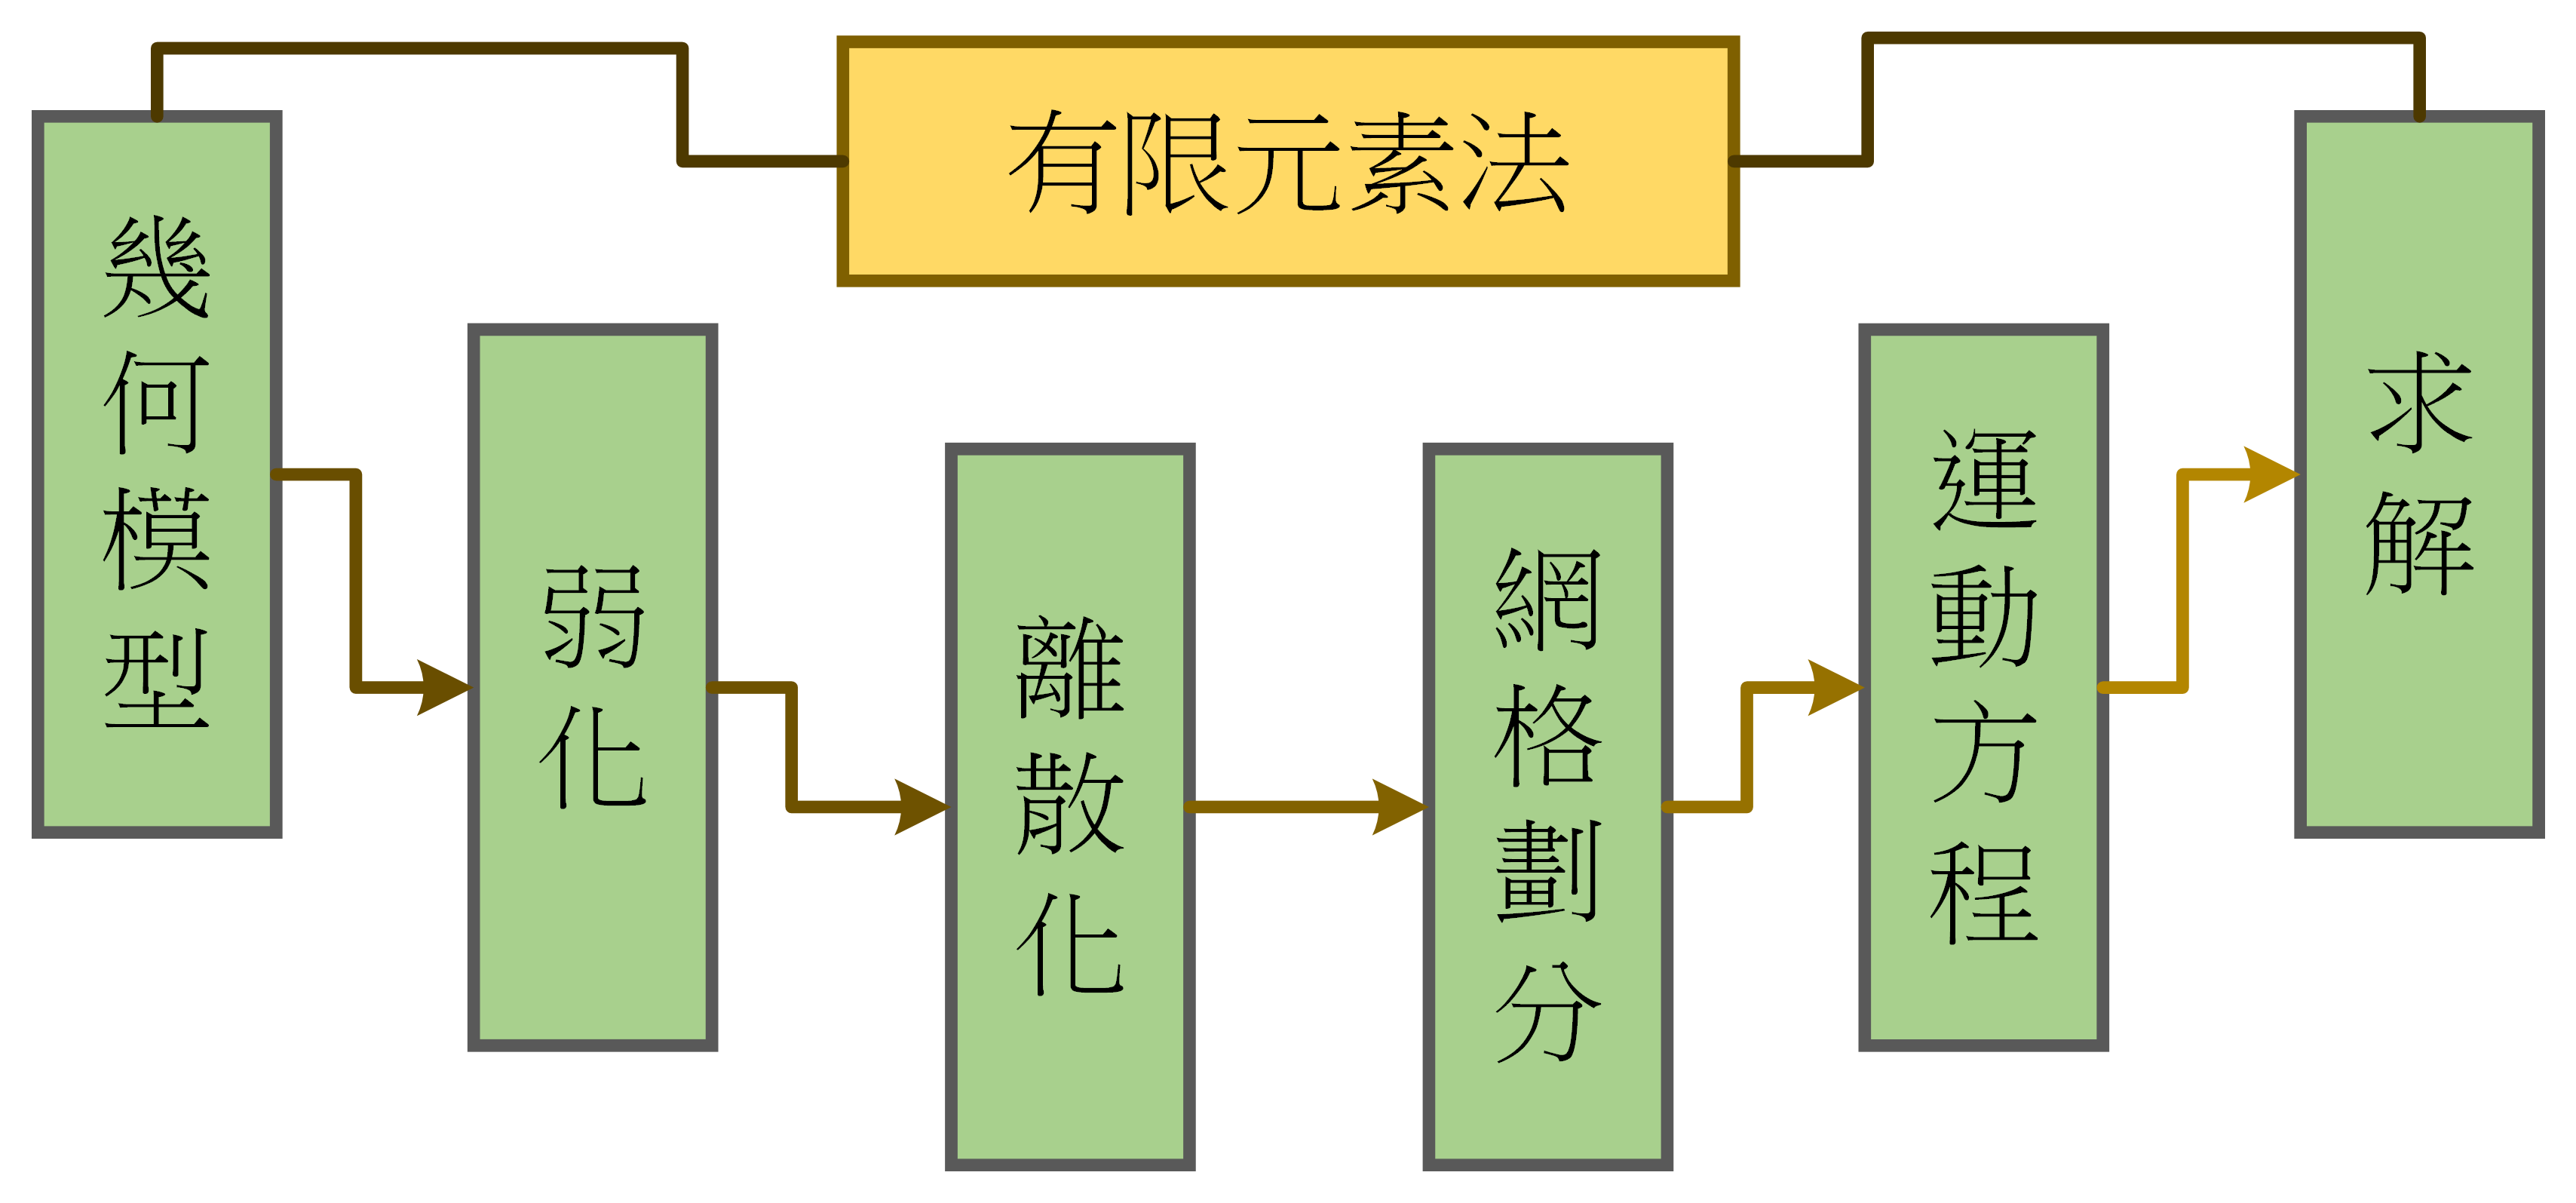
\includegraphics[width=15cm]{有限元素法分析流程}
\caption{\Large 有限元素法分析流程}\label{有限元素法分析流程}
\end{center}
\end{figure}
\begin{itemize}
\item 幾何模型:透過繪圖軟體將模型畫出,將模型以數據方式在電腦裡呈現二維或三維的外觀,便於軟體將其代入且計算。
\item 離散化及元素劃分:將物理系統或結構等連續變量通過計算轉換為數格元素的過程,對於複雜的連續變量,需先進行弱化的動作,才能進行離散化將其轉變為各個元素,此動作由分析軟體內部公式計算。
\item 導入函數並組成代數方程: 模型或問題不同,力學性質及物理方程相應的關係式(應力、應變、變形、熱傳等)也會跟著變化,因此需要根據對應的問題分別導入不同的函數,需在軟體內設定問題,讓其可以對特定問題進行求解,此動作為設計者提問,軟體負責計算。
\item 求解方程:在經過有限元素法分析後,將會在每個表面得知各元素的受力情況,設計者可以根據此數據了解到模型的受力狀態或位移及負載等相關訊息,以利於後續的設計或生產。
\end{itemize}
\newpage
